\documentclass[a4paper]{article}
\usepackage[utf8]{inputenc}
\usepackage{amsmath}
\usepackage{amssymb}
\usepackage{mathtools}
\usepackage{amsfonts}
\usepackage{lastpage}
\usepackage{tikz}
\usepackage{float}
\usepackage{textcomp}
\usetikzlibrary{patterns}
\usepackage{pdfpages}
\usepackage{gauss}
\usepackage{fancyvrb}
\usepackage[table]{colortbl}
\usepackage{fancyhdr}
\usepackage{graphicx}
\usepackage[margin=2.5 cm]{geometry}

\definecolor{listinggray}{gray}{0.9}
\usepackage{listings}
\lstset{
	language=,
	literate=
		{æ}{{\ae}}1
		{ø}{{\o}}1
		{å}{{\aa}}1
		{Æ}{{\AE}}1
		{Ø}{{\O}}1
		{Å}{{\AA}}1,
	backgroundcolor=\color{listinggray},
	tabsize=3,
	rulecolor=,
	basicstyle=\scriptsize,
	upquote=true,
	aboveskip={0.2\baselineskip},
	columns=fixed,
	showstringspaces=false,
	extendedchars=true,
	breaklines=true,
	prebreak =\raisebox{0ex}[0ex][0ex]{\ensuremath{\hookleftarrow}},
	frame=single,
	showtabs=false,
	showspaces=false,
	showlines=true,
	showstringspaces=false,
	identifierstyle=\ttfamily,
	keywordstyle=\color[rgb]{0,0,1},
	commentstyle=\color[rgb]{0.133,0.545,0.133},
	stringstyle=\color[rgb]{0.627,0.126,0.941},
  moredelim=**[is][\color{blue}]{@}{@},
}

\lstdefinestyle{base}{
  emptylines=1,
  breaklines=true,
  basicstyle=\ttfamily\color{black},
}

\pagestyle{fancy}
\def\checkmark{\tikz\fill[scale=0.4](0,.35) -- (.25,0) -- (1,.7) -- (.25,.15) -- cycle;}
\newcommand*\circled[1]{\tikz[baseline=(char.base)]{
            \node[shape=circle,draw,inner sep=2pt] (char) {#1};}}
\newcommand*\squared[1]{%
  \tikz[baseline=(R.base)]\node[draw,rectangle,inner sep=0.5pt](R) {#1};\!}
\newcommand{\comment}[1]{%
  \text{\phantom{(#1)}} \tag{#1}}
\def\el{[\![}
\def\er{]\!]}
\def\MeanN{\frac{1}{N}\sum^N_{n=1}}
\cfoot{Page \thepage\ of \pageref{LastPage}}
\DeclareGraphicsExtensions{.pdf,.png,.jpg}
\author{Nikolaj Dybdahl Rathcke (rfq695)}
\title{Machine Learning \\ Assignment 2.1}
\lhead{Machine Learning}
\rhead{Assignment 2.1}

\begin{document}
\maketitle

\section{Logistic regression}
\subsection{Cross-entropy error measure}
\textbf{(a)} \\
The maximum likelihood selects a hypthesis $h$ which maximizes a probability. We can rewrite this so it minimizes it instead:
\begin{align*}
-\frac{1}{N}\ln\left( \prod_{n=1}^N P(y_n|x_n) \right) = \frac{1}{N}\sum_{n=1}^N \ln\left( \frac{1}{P(y_n|x_n)} \right)
\end{align*}
We know $y$ only takes values in $\{-1,1\}$ and we know that $P(y_n|x_n)=h(x_n)$ when $y_n=1$ and $1-h(x_n)$ in the other case. Since we want to minimize this quantity, we can treat it as an error measure, so we can write $E_{in}(w)$ as:
\begin{align*}
E_{in}(w)&=\frac{1}{N}\sum_{n=1}^N \ln\left( \frac{1}{P(y_n|x_n)} \right) \\
&=\frac{1}{N}\sum_{n=1}^N \el y_n=1 \er \ln\left( \frac{1}{h(x_n)} \right) + \el y_n=-1 \er \ln\left( \frac{1}{1-h(x_n)} \right) \\
&=\sum_{n=1}^N \el y_n=1 \er \ln\left( \frac{1}{h(x_n)} \right) + \el y_n=-1 \er \ln\left( \frac{1}{1-h(x_n)} \right)
\end{align*}
We can do the last step since we are minimizing and dividing the value by $N$ will not change the $w$ we find, and this is what we wanted to show.\\
\\
\textbf{(b)} \\
Remember $\theta(s)=\frac{e^s}{1+e^s}$, so we have the following limits:
\begin{align*}
  \lim_{s\rightarrow \infty}&=1 \\
  \lim_{s\rightarrow -\infty}&=0 \\
  \comment{From both sides}  \lim_{s\rightarrow 0}&=1/2
\end{align*}
In equation (3.9), the term $e^{-y_nw^Tx_n}$ is deciding for how small the in-sample error is. Thus we want $y_nw^Tx_n$ to be as large as possible so the entire term is as small as possible. This means we want $w^Tx_n$ to be the same sign as $y_n$. \\
For the equation we found in (a), if $y_n=1$, we want $h(x)=\theta(w^Tx_n)$ to be large and positive as it contributes less to the sum than if it is small (see limits). When $y_n=-1$, we want $1-h(x)$ to be large, which means we want $h(x)$ to be as small as possible (large and negative). \\
So for both equations we want them to be to be the same sign and they grow in same fashion, the task of minimizing are equivalent.

\subsection{Logistic regression loss gradient}
Equation (3.9) in the textbook says:
\begin{align*}
E_{in}(w)=\MeanN \ln(1+e^{-y_n w^T x_n})
\end{align*}
We can take the derivative, of this, by first applying the chain rule and get:
\begin{align*}
\nabla E_{in}(w)&=\MeanN \frac{1}{1+e^{-y_n w^T x_n}}(-y_nx_ne^{-y_n w^T x_n}) \\
&=-\MeanN \frac{y_nx_ne^{-y_n w^T x_n}}{1+e^{-y_n w^T x_n}} \\
&=-\MeanN \frac{y_nx_n}{1+e^{y_n w^T x_n}} \\
&=\MeanN -y_nx_n\theta(-y_nw^Tx_n)
\end{align*}
And we have showed the derivative. \\
When $y_n$ and $w^Tx_n$ have different signs (they are misclassified)), the product $s=-y_nw^Tx_n$ becomes positive. Our limits from (1.1) tells us that the value $\theta(s)$ must lie in $(0.5,1)$. When $y_n$ and $w^Tx_n$ have the same sign (classified correctly), then $s=-y_nw^Tx_n$ is negative and our limits tell us they must lie in $(0, 0.5)$. Thus, misclassified examples contribute more to the gradient.

\subsection{Logistic regression implementation}
The logistic regression algorithm (Example 3.3 in the textbook) has been implemented in \texttt{src/logistic\_regr.py}. Running the file will report the parameters we found as well as the error on the training and test set:
\begin{verbatim}
Parameters for the model:
[-0.00813814 -0.02809434]

Error on training set with found parameters:
0.451612903226

Error on test set with found parameters:
0.384615384615
\end{verbatim}
Where a successfull prediction is when the probability if more than $0.5$ for the right classication and if not, it is a misprediction.

\section{Linear least squares}
\subsection{}
To implement this, since we expect the canonball to fly in a parabola like fashion, we use $d=2$. The method \texttt{leastSquares} in \texttt{least\_squares.py} implements this by constructing the matrix:
\begin{align*}
A =
\begin{bmatrix}
0 & 0 & 1 \\
x_1^2 & x_1 & 1 \\
\vdots & \vdots & \vdots \\
x_8^2 & x_ 8 & 1
\end{bmatrix}
\end{align*}
The first line is added because we also know the position of the cannon (and the height is $0$ in that point). We can find the parameters by calculating
\begin{align*}
w = (A^TA)^{-1}A^Ty
\end{align*}
where $y$ is our measured height and $x$ is the horizontal distance from the cannon. This yields the parameters:
\begin{verbatim}
Parameters from least squares with d=2:
[-0.97880952  9.98280952 -0.466     ]
\end{verbatim}
which is equal to the formula $f(x)=-0.9788x^2+9.9828x-0.466$.

\subsection{}
To estimate how far from the cannon Baron Münchhausen will fall, we simply solve for $x$ when the $f(x)$ is equal to zero. This gives the following results:
\begin{align*}
x\approx 0.0469 \mbox{  or  } x=10.152
\end{align*}
since the first solution is the cannon's position, the second solution is where Baron Münchhausen will fall, so at distance $10.152$.

\subsection{}
The following figure shows the comparison between the measured points and the result from using the least squares method:
\begin{center}
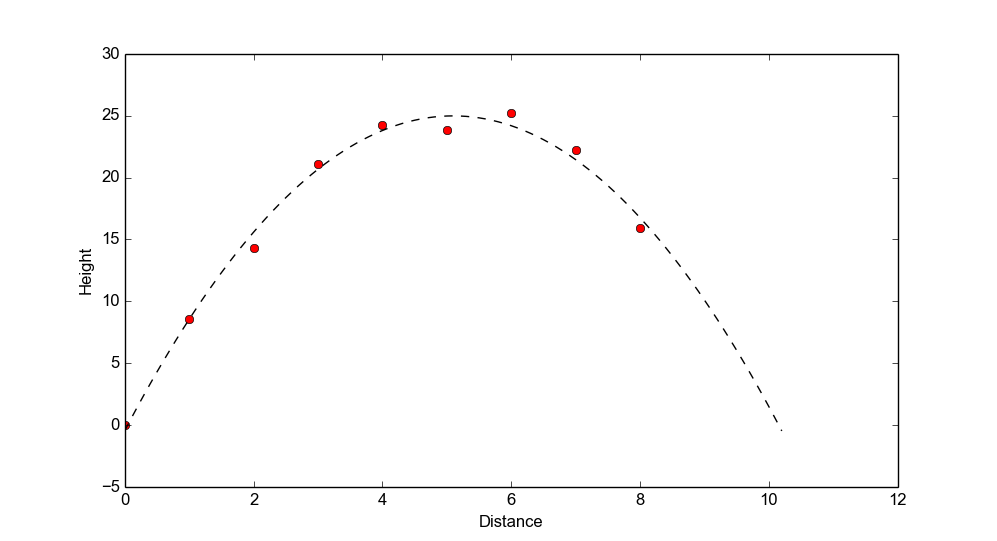
\includegraphics[scale=0.5]{f1}
\end{center}
Where the red points are the measured points and the dotted line is our estimation of a function. The estimation has very little noise.

\end{document}
